\documentclass[12pt,oneside]{memoir}

\usepackage{helvet}
\usepackage[top=3cm, bottom=2cm, left=2cm, right=2cm]{geometry}
\usepackage{amsmath, amsthm, amssymb}
\usepackage{wrapfig}
\usepackage{graphicx}
\usepackage{verbatim}
\usepackage[version=3]{mhchem}
\usepackage{ifthen}

\setlength{\headheight}{52pt}

\setlength\headsep{8mm}
\parindent 0mm

\renewcommand{\labelitemi}{$ $}

\newcommand{\onehalf}{\frac{1}{2}}
\newcommand{\del}{\nabla}
\newcommand{\cross}{\times}


\newenvironment{frcseries}{\fontfamily{frc}\selectfont}{}
\newcommand{\textcrsv}[1]{{\frcseries#1}}

\newcommand{\xhat}{\mathbf{\hat{x}}}
\newcommand{\yhat}{\mathbf{\hat{y}}}
\newcommand{\zhat}{\mathbf{\hat{z}}}

\newcommand{\rhat}{\mathbf{\hat{r}}}
\newcommand{\thetahat}{\mathbf{\hat{\theta}}}
\newcommand{\phihat}{\mathbf{\hat{\phi}}}

\newcommand{\shat}{\mathbf{\hat{s}}}

\newcommand{\curly}[1]{\text{\textcrsv{#1}}}
\newcommand{\curlyr}{\text{\textcrsv{r}}}
\newcommand{\curlyL}{\text{\textcrsv{L}}}
\newcommand{\curlyrhat}{\hat{\text{\textcrsv{r}}}}
\newcommand{\nhat}{\mathbf{\hat{n}}}

\newcommand{\ket}[1]{|#1\rangle}
\newcommand{\bra}[1]{\langle#1|}

\newcommand{\nextstep}{\hspace{4mm} \Rightarrow \hspace{4mm}}

\newcommand{\pvector}[1]
{
	\begin{pmatrix} #1 \end{pmatrix} 
}

\newcommand{\spinup}
{
	\begin{pmatrix} 
		1 \\
		0
	\end{pmatrix}
}
\newcommand{\spindown}
{
	\begin{pmatrix} 
		0 \\
		1
	\end{pmatrix}
}
\newcommand{\sigmax}
{
	\begin{pmatrix} 
		0 & 1 \\
		1 & 0
	\end{pmatrix}
}
\newcommand{\sigmay}
{
	\begin{pmatrix} 
		0 & -i \\
		i & 0
	\end{pmatrix}
}
\newcommand{\sigmaz}
{
	\begin{pmatrix} 
		1 & 0 \\
		0 & -1
	\end{pmatrix}
}

\makeatletter
\def\tensor#1{\protect\@ontopof{#1}{\leftrightarrow}{1.15}\mathord{\box2}}
\def\overstar#1{\protect\@ontopof{#1}{\ast}{1.15}\mathord{\box2}}
\def\overdots#1{\protect\@ontopof{#1}{\cdots}{1.0}\mathord{\box2}}
\def\overcirc#1{\protect\@ontopof{#1}{\circ}{1.2}\mathord{\box2}}
\def\loarrow#1{\protect\@ontopof{#1}{\leftarrow}{1.15}\mathord{\box2}}
\def\roarrow#1{\protect\@ontopof{#1}{\rightarrow}{1.15}\mathord{\box2}}

\def\@ontopof#1#2#3{%
{\mathchoice
{\@@ontopof{#1}{#2}{#3}\displaystyle\scriptstyle}%
{\@@ontopof{#1}{#2}{#3}\textstyle\scriptstyle}%
{\@@ontopof{#1}{#2}{#3}\scriptstyle\scriptscriptstyle}%
{\@@ontopof{#1}{#2}{#3}\scriptscriptstyle\scriptscriptstyle}%
}}
\def\@@ontopof#1#2#3#4#5{%
\setbox0=\hbox{$#4#1$}%
\setbox1=\hbox{$#5#2$}%
\setbox2=\hbox{}\ht2=\ht0 \dp2=\dp0 %
\ifdim\wd0>\wd1 %
\setbox1=\hbox to\wd0{\hss\box1\hss}%
\mathord{\rlap{\raise#3\ht0\box1}\box0}%
\else   %
\setbox1=\hbox to.9\wd1{\hss\box1\hss}%
\setbox0=\hbox to\wd1{\hss$#4\relax#1$\hss}%
\mathord{\rlap{\copy0}\raise#3\ht0\box1}%
\fi
}
\makeatother

\begin{comment}
\begin{center}
	\includegraphics[width=100mm]{fig_qual_TERM.jpg}
\end{center}

\begin{description}

  \setlength{\parskip}{0pt}
  \setlength\labelwidth{-4pt}

  \item[(a)] 
  \item[(b)] 
\end{description}

\end{comment}


\title{MICE Global Track Reconstruction Specification}
\date{}

\chapterstyle{article}

\maxsecnumdepth{subsection}
\maxtocdepth{subsection}

\begin{document}

\frontmatter
\maketitle
\begin{center}

\chapter{MAUS Work Specification Document}

\end{center}
\section{Change History}
\begin{center}
	\begin{tabular}{|l|p{0.615\textwidth}|l|l|p{2cm}} %| L | L | L | L |
		\hline
		\textbf{Version} & \textbf{Changes} & \textbf{Author} & \textbf{Date} \\
		\hline
		1 & First draft & C. Rogers & 06/01/2012 \\
		\hline
		2 & \LaTeX\ draft with class hierarchy & P. Lane & 14/02/2012 \\
		\hline
		3 & Section reorganization. Polynomial map and task details. & P. Lane & 16/02/2012 \\
		\hline
		4 & Dot-derived class hierarchy diagram.  & P. Lane & 21/02/2012 \\
		\hline
	\end{tabular}
\end{center}
\section{Project Summary}
\begin{center}
	\begin{tabular}{|l|p{0.798\textwidth}|p{1cm}} %| L | L | L | L |
		\hline
		\textbf{Project Title} & Global Reconstruction \\
		\hline
		\textbf{Main Issue} & Create a global track reconstruction tool.\\
		\hline
		\textbf{Subtask Issues} & \\
		\hline
		\textbf{Project Lead} & P. Lane \\
		\hline
		\textbf{Project} 		 & A. Blondel \\
		\textbf{Supervisor(s)} & C. Rogers \\
		\hline
		\textbf{Associated} & \\
		 \textbf{Manpower} & \\
		\hline
	\end{tabular}
\end{center}

\newpage

\tableofcontents

\mainmatter

\part{Overview of Work}

\chapter{Motivation and Overview}

\section{Project Goal}

The MICE collaboration, seeks to:
\begin{itemize}
\renewcommand{\labelitemi}{$\bullet$}
  \item measure phase space variables position, time, momentum and energy at different planes along the beam axis of the experiment;
  \item identify the particle species of particles traversing the experiment.
\end{itemize}

One seeks to compare the two sets of variables to perform certain physics analyses such as calculating beam properties like emittance. In addition, one seeks to propagate these variables through the experiment, for example to perform detector alignment in the presence of fields or to measure the effect of physics processes in the cooling channel (e.g. multiple scattering at absorbers).\\

The position and momentum is measured at the trackers, while time is measured at fast time of flight detectors upstream and downstream of the experiment. Additionally some detectors have been placed into the accelerator specifically to determine particle species, namely the KL, EMR and Cerenkov detectors. The reconstruction of individual detectors is the task of the detector working groups, under joint supervision of the MAUS project manager and detector working group managers.\\

The global reconstruction task is to connect together the individual measurements of each detector into a global track. Typically, one would seek to make global tracks that conform as closely as possible to the measurements made by each individual detector.

\section{Use Cases}

Here I include a few sample analyses (not exhaustive) that one might want to make of a global reconstruction algorithm:

\begin{itemize}
\renewcommand{\labelitemi}{$\bullet$}
  \item Generate phase space vectors at the input and output of MICE. Reject all particles that are not muons or do not traverse the experiment. Calculate the change in 4D emittance.
  \item Generate phase space vectors at the input and output of MICE. Reject all particles that are not muons or do not traverse the experiment. Calculate the change in longitudinal (time-energy) emittance.
  \item Calculate time and energy at the input and output of MICE. Look at the energy change vs time relationship for individual particles and verify that the energy change in RF cavities is correct.
  \item Generate phase space vectors at the input of MICE using only upstream detectors. Apply some cut to the data to reject particles that do not conform to an ideal beam distribution. Generate phase space vectors at the output of MICE and calculate the emittance change.
  \item Calculate a phase space vector at the input to MICE using only the upstream tracker. Propagate it to the output of MICE. Calculate a phase space vector at the output to MICE using only the downstream tracker. Compare the residuals to understand whether there is a bias in the reconstruction of events (caused by e.g. detector or magnet misalignment).
  \item Calculate phase space vectors at the input to MICE. Look at those that are not transmitted to the output of MICE. Seek to understand the aperture of the cooling channel.
  \item Calculate beam purity in the MICE beamline. Seek to optimise magnet settings for a pure muon beam.
\end{itemize}

And so on...

\chapter{Specification}

The global reconstruction shall generate a track consisting of a set of phase space vectors with the following information.
\begin{itemize}
\renewcommand{\labelitemi}{$\bullet$}
   \item x
   \item y
   \item z
   \item t
   \item px
   \item py
   \item pz
   \item energy
  \item Most favoured particle type (pid)
 \end{itemize}

Additionally the global reconstruction shall return errors for the phase space vector

\begin{itemize}
\renewcommand{\labelitemi}{$\bullet$}
   \item The error matrix on the phase space variables u=(x,y,t,px,py,energy) � that is the matrix of errors and correlations where each element of the matrix vij are of the form Cov(ui, uj) where Cov() is the covariance for the (multidimensional) error probability distribution function.
   \item Probability that the particle is an electron, muon, pion or �something else� \emph{is that right? Or should we have errors on mass? Or something else?}
 \end{itemize}

The global reconstruction routines shall work with any set of detectors, for example it should be possible to do �only upstream�, �only downstream� and �combined� analyses; and if a detector is removed for maintenance we should be able to work without.\\

The global reconstruction shall reconstruct tracks at user-defined positions along the beamline.
The global reconstruction shall not have a preferred frame of reference.\\

\begin{itemize}
\renewcommand{\labelitemi}{$\bullet$}
   \item we will probably end up working in engineering coordinates with x-axis being the beam axis
   \item we might want to include dipoles in the track fitting routine
 \end{itemize}

The global reconstruction shall reconstruct tracks passing through

\begin{itemize}
\renewcommand{\labelitemi}{$\bullet$}
   \item Material
   \item Solenoidal fields
   \item Quadrupole fields
   \item RF fields
   \item Dipoles
 \end{itemize}

\chapter{Implementation}

\section{Optics Model}

The optics model is embodied in the transfer map. Two different models are foreseen:  polynomial expansion and Runge-Kutta. Neither of these methods accounts for scattering in materials. An additional procedure must be used to deal with these non-linear momentum changes.

\subsection{Polynomial Transfer Map}

The polynomial transfer map is an expansion of each coordinate in the final phase space vector as a multivariate polynomial in terms of the initial phase space vector coordinates. The transfer map then comes in the form of a matrix of polynomial coefficients $P_{ij}$. To transform a phase space vector, it is first expanded into a vector of polynomial variable terms
\[
	\pvector{t, E, x, p_x, y, p_y} \rightarrow \pvector{1, t, E, x, p_x, y, p_y, t^2, t E, t x, t p_x, \dots}
\]
 and then operated on by the coefficient (transfer) matrix:
\[
	\pvector{t_f \\ E_f \\ x_f \\ p_{x_f} \\ y_f \\ p_{y_f}} =
	\begin{pmatrix}
		P_{11} &\dots & \dots & \dots & \dots & P_{1N} \\
		P_{21} & \ddots & & & & \vdots \\
		P_{31} & & \ddots & & & \vdots \\
		P_{41} & & & \ddots && \vdots \\
		P_{51} & & & & \ddots & \vdots \\
		P_{61} & \dots & \dots & \dots & \dots & P_{6N}
	\end{pmatrix}
	\pvector{1 \\ t_i \\ E_i \\ \vdots \\ t_i p_{x_i} \\ \vdots}_\cdot
\]

The beam envelopes can be transported by a similarity transform by a matrix formed from the first-order elements of the transfer matrix:
\[
	\begin{pmatrix}
		<t t> & \dots & <t p_y> \\
		\vdots & \ddots & \vdots \\
		<p_y t> & \dots & <p_y p_y>
	\end{pmatrix}=
	\begin{pmatrix}
		P_{12} & \dots & P_{17} \\
		\vdots & \ddots & \vdots \\
		P_{62} & \dots & P_{67}
	\end{pmatrix}
	\begin{pmatrix}
		<t t> & \dots & <t p_y> \\
		\vdots & \ddots & \vdots \\
		<p_y t> & \dots & <p_y p_y>
	\end{pmatrix}
	\begin{pmatrix}
		P_{12} & \dots & P_{17} \\
		\vdots & \ddots & \vdots \\
		P_{62} & \dots & P_{67}
	\end{pmatrix}^T
\]

\subsection{Runge-Kutta Transfer Map}

The Runge-Kutta method calculates incremental vector deltas over uniform intervals along the beam axis. The deltas are then integrated to produce the final vector from the initial vector. Details of the algorithm can be found online or in the literature.\\

Additional care will need to be taken when transporting particles backwards through the lattice as Runge-Kutta incorrectly handles energy gain in materials. Considering that multiple scattering is also not handle automatically, it is apparent that only free-space transport will be handled by the Runge-Kutta algorithm. Transport through materials will be handled separately.\\

The beam envelope is transported by calculating a transfer matrix between two incremental steps of the vector and performing a similarity transformation as was described in \emph{Polynomial Transfer Map}.

\subsection{Calculation of the Transfer Matrix}

\subsubsection{Numerical Differentiation of Tracking}

The transfer matrix can be calculated by numerically differentiating tracking output. Say we have a 2D transfer matrix in $(x,p_x)$. We propagate tracks by integration of the usual equations of motion. Let us propagate the following three tracks
\[
		u_a = (x, p_x)
\]
\[
		u_b = (x+dx, p_x)
\]
\[
		u_c = (x, p_x+dp)
\]
Here $u_a$ is just the central track. Then using the defining relationship for a transfer matrix,
\[
		u_2=M_{12}u_1
\]
we can write
\[
		u_{b,2} =M_{12} u_{b,1}
\]
\[
		u_{c,2} = M_{12} u_{c,1}
\]
which is a simultaneous equation with unknowns as the terms of $M$, that can be solved using  common simultaneous equation techniques. The algorithm generalises to an arbitrary dimension phase space.

\subsubsection{Linear Least Squares (first order correction)}

The second order correction can be made by propagating more tracks. Let's now propagate
\[
		u_b = (x+dx, p_x)
\]
\[
		u_c = (x, p_x+dp)
\]
\[
		u_d = (x-dx, p_x)
\]
\[
		u_e = (x, p_x-dp)
\]
Then instead of searching for the transfer matrix using a first order differentiation as above, we can find the tracks using a linear least squares fit. This should eliminate errors due to second order derivatives from the transfer matrix calculation, at a cost of doubling the number of tracks that must be transported.

\subsubsection{Direct Integration}

It is additionally possible to derive differential equations for the transfer matrix elements directly, for example, by taking the usual equations of motion and integrating them using standard techniques. This may be faster to run and will require fewer control parameters (a distance and a time).

\section{Reconstruction}

The fundamental algorithm that is proposed for track reconstruction is to take information yielded by each detector, together with estimated errors, and find the track that minimises the sum of the residuals (difference between the model prediction and the measurement from the detector) of each measurement, normalised to the errors on the measurement.  In general, two algorithms are foreseen:

\begin{itemize}
\renewcommand{\labelitemi}{$\bullet$}
   \item An algorithm that propagates the tracks and associated error matrix between detectors
   \item A minimisation routine that minimises the errors given the tracks
 \end{itemize}

Several different algorithms can be foreseen; one task of the Global Reconstruction is to determine a framework in which different algorithms can be implemented without major infrastructure changes.\\

\subsection{Track and Error Propagation}

In the paraxial approximation, tracks propagate according to an equation like
\[
	u_2 = M_{12} u_1
\]
where $u_1$, is the phase space vector at some $z$ position $z_1$, $u_2$ is the phase space vectors at some $z$ position $z_2$ and $M_{12}$ is the transfer matrix that propagates particles from $z_1$ to $z_2$ The error matrix propagates like
\[
	V_2 = M_{12} V_1 M_{12}^T
\]
where T superscript denotes the transpose matrix, $V_1$ denotes the error matrix at $z_1$, $V_1$ denotes the error matrix at $z_1$. (These relationships can be derived, see for example Chris Rogers thesis chapter 3, available on MICE website).
We seek to minimise the sum of the $\chi^2$ over the $i$ measurements, defined by
\[
		\sum \chi_i^2 = \sum u_i \curly{E}_{i-1} u_i^T
\]
where the $i$ subscript indicates that the values are calculated at the position of the $i$th detector. $\curly{E}_i$ is the error matrix associated with a particular detector.
Possibly can linearise this problem completely (i.e. express as linear sum of some seed value) to make linear least squares possible.\\

\subsubsection{Propagation through Material}

The presence of material in the beamline introduces energy loss to the track and creates noise that increases errors.\\

Tracks propagate through material losing energy according to the Bethe Bloch relationship.
Error matrices propagate through material in the thin material approximation as pure scattering and energy straggling.\\

From the Particle Data Group's July 2010 \emph{Particle Physics Booklet}...\\

For a gaussian distribution of small scattering angles, the width of the gaussian is
\[
	\theta_0 = \frac{13.6 \text{MeV}}{\beta_c p} z \sqrt{x/X_0} \left[1+0.038 \ln (x/X_0)\right],
\]
where $p$, $\beta_{c}$, and $z$ are the momentum, velocity, and charge number of the incident particle; and $x/X_0$ is the thickness of the scattering medium in radiation lengths.\\

The mean energy deposit by an ionizing particle when energy transfers are restricted to $T \le T_\text{cut} \le T_\text{max}$ is
\[
	\left. -\frac{dE}{dx} \right|_{T<T_\text{cut}} = K_z^2 \frac{Z}{A} \frac{1}{\beta^2}
	\left[\onehalf \ln \frac{2 m_e c^2 \beta^2 \gamma^2 T_\text{cut}}{I^2} - \frac{\beta^2}{2}
	\left(1+\frac{T_\text{cut}}{T_\text{max}}\right)-\frac{\delta}{2}\right]
\]

\subsection{Score Function Minimisation}

As discussed above, the reconstruction routine requires minimisation of the sum of the chi-squared values, $\sum \chi_i^2$. Various minimisation routines exist. It is foreseen that two routines will be investigated initially: Minuit and Kalman Filter.

\subsubsection{Minuit Minimisation}

Minuit is the algorithm, packaged with ROOT, that allows for solving of fairly general minimisation problems. It has a fairly tractable interface (see TMinuit documentation in ROOT) although it is probably not optimal for our problem. However, the majority of the optimisation has been done already as it is built-in to ROOT.

\subsubsection{Kalman Filter Minimisation}

The Kalman filter technique may be a more optimal solution. This algorithm has been proposed for use by the tracker group.\\

The Kalman filter would work in the context of track reconstruction by predicting subsequent particle event coordinates and calculating a weighted average between the prediction and the actual measurement from the detector. The transfer matrix is given, and the last weighted average is propagated back through the lattice to produce a final trajectory.\emph{Is this last part right?}

\subsubsection{TOF Iteration (\emph{Better Name?})}

The TOF iteration takes advantage of the fact that the TOFs reconstruct longitudinal phase space quite accurately, and that longitudinal phase space is approximately independent of longitudinal phase space (cf Mark Rayner thesis). The TOF iteration
1. reconstructs momentum from measured time of flight
2. generates a transfer matrix for this momentum
3. uses the generated transfer matrix to calculate transverse phase space parameters
4. recalculates momentum using transverse phase space parameters

\subsubsection{Other Minimisation Techniques}

There is a rich literature in minimisation algorithms dating back to the era of Newton. Neural networks, simulated annealing, etc.

\subsection{Seed Finding}

All the minimisation routines discussed above are iterative routines. In most cases, the tracker reconstruction will deliver a seed for the global reconstruction. An additional time parameter will be required. This can be calculated analytically assuming no energy loss between the tracker and the nearest time of flight detector.
If the tracker is not in use or reconstruction of tracks with no tracker hit is required, it may be sufficient to assume a paraxial particle.

\section{Particle Identification}

Particle identification can be treated in either of two ways. The simplest method is to specify a list of candidate particles and pick out the best fit given certain parameters. One may also be able to use mass as a free parameter in the track fitting.

\subsection{Candidate Particles}

This method performs track fitting with three candidate particle types: electron, muon, and pion. The most favoured particle type is that which fits the input variables in the best approximation.\\

A second round of fitting adding results such as light yield in the Cerenkovs may then improve the pid.

\subsection{Mass as a Free Parameter}

It may also be possible to use mass as a free parameter in the track finding. The algorithms described above are sufficiently general that they can support track finding with any mass. Charge will be assumed to be +1 or -1 according to the beamline polarity.

\subsection{Any other PID routines?}

\section{Class Hierarchy}

Figure 1.1 shows the proposed, main class hierarchy for track reconstruction. The two interfaces TransferMap and TrackFitter provide the required implementation flexibility which is detailed in figure 1.2. The particular track fitting algorithm can be specified in the configuration file and the appropriate class instance will be instantiated.

\begin{figure}
\centering
\hspace*{\fill}
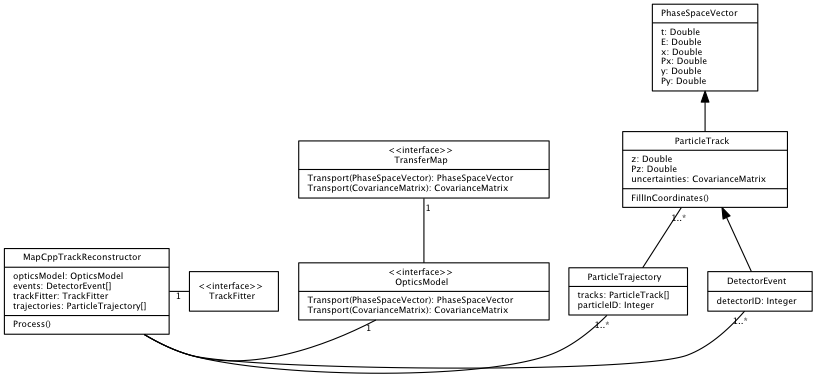
\includegraphics[width=180mm]{class_hierarchy_main.png}
\hspace*{\fill}
\caption{Main track reconstruction class hierarchy} \label{fig:mult1}
\end{figure}

\begin{figure}
\centering
\hspace*{\fill}
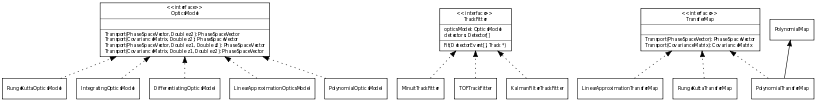
\includegraphics[width=180mm]{class_hierarchy_interfaces.png}
\hspace*{\fill}
\caption{Track reconstruction interface details} \label{fig:mult1}
\end{figure}

\section{Task Breakdown}

\subsection{Data Structures}

Define input and output data structures. It is crucial to get this flushed out early on so that the detector groups know what is needed. Referring to the class diagram, this would involve implementing PhaseSpaceVector (exists already), ParticleTrack, DetectorEvent, and ParticleTrajectory.

\subsection{Interfaces}

Defining the OpticsModel and TransferMap interfaces.

\subsection{Polynomial Transfer Map}

Convert existing PolynomialVector into three separate classes: PolynomialMap, PolynomialVector, and LeastSquaresOpticsModel. LeastSquaresOpticsModel would become an implementation of the OpticsModel interface. The PolynomialTransferMap class will be the first TransferMap  implementation, and will also be a subclass of PolynomialMap.

\subsection{Basic Minuit Track Fitter}

The TrackFitter implementation MinuitTrackFitter will be created and tested with just fields (no materials).

\subsection{Basic Track Reconstructor}

This will likely be created in tandem with the Minuit Track Fitter to serve as an interface for testing the reconstruction. This task is to create a "map" in the Python Map/Reduce flow structure that can be inserted into the chain of execution of a MAUS simulation or live run.

\subsection{Minuit Material Effects}

Materials will be added to the transfer matrix based transport algorithm.

\subsection{Differentiating Optics Model}

The DifferentiatingOpticsModel class will be created that conforms to the OpticsModel interface. it will be tested and compared to the least squares optics model.

\subsection{Integrating Optics Model}

The IntegratingOpticsModel class will be created that conforms to the OpticsModel interface. It will be tested and compared to the differentiating and least-squares optics models.

\subsection{Runge-Kutta Transfer Map}

The RungeKuttaOpticsModel class will be created that conforms to the OpticsModel interface. This may be as simple as simple creating a RungeKuttaTransferMap instance the model does not require a matrix representation. The RungeKuttaTransferMap class will be implemented, conforming to the TransferMap interface. Again, no material effects will be included at this stage.

\subsection{Runge-Kutta Material Effects}

Materials will be incorporated into the Runge-Kutta transport algorithm.

\subsection{Kalman Filter}

The TrackFitter implementation KalmanFilterTrackFitter will be created, tested, and compared with the Minuit track fitter.

\subsection{TOF Track Fitter}

The TrackFitter implementation TOFTrackFitter will be created, tested, and compared with the Minuit and Kalman filter track fitters.

\section{Existing Code and Location of New Code}

\section{Potentially Conflicting Work}

\part{MAUS Overview and Requirements}

MAUS is an analysis tool designed for the reconstruction and analysis of the Muon Ionisation Cooling Experiment.
The MAUS project uses a number of tools to manage code and the development process. Issue trackers are used to monitor development of new features and log any issues arising such as bugs. Code is stored using Version Control System (VCS). Communication between the development team is achieved using mailing lists, regular phone conferences etc. Code quality is assured by a set of style requirements, testing requirements, documentation of code and regular code reviews.
These tools are documented here for convenience, but additional documentation can be found on the MAUS website http://micewww.pp.rl.ac.uk/projects/maus/wiki/MAUSDevs. Where there is a conflict, the MAUS website takes precedence as this is more likely to be updated.

\section{Issue Tracking}

The Redmine issue tracking system is used to monitor development of new features and log any issues arising such as bugs. Any information pertaining to the features in this document shall be stored in the relevant issues on that system. Redmine issues can be found by following the Issues link on the MAUS website.

\section{Code Version Control}

Code is controlled using the Bazaar Distributed Version Control System (bzr). Before writing code, developers shall checkout a copy of the maus trunk (lp:maus). Developers shall then make their own development branch on launchpad. Code shall be pushed regularly to this development branch (typically nightly). Every release, the MAUS trunk shall be merged with the development branch to ensure that development is performed against the latest MAUS version.
Further guidance on bzr usage can be found on the MAUS wiki.

\section{Communication}

Communication is performed using mailing lists and fortnightly phone meetings. All developers should be subscribed to the following mailing lists:
mice-software
maus-devs
maus-users
Where possible, developers shall attend the fortnightly phone meetings, as announced on the mice-software mailing lists.

\section{Code Quality}

Code quality is ensured by a number of tools. Code must be commented and conform to certain style requirements. All code must have appropriate regression tests. Documentation must be created or updated as appropriate. Code may be reviewed by one or more developers before submission.
The workflow that ensures code quality is controlled by the workflow field in the issue tracker. As code moves through the workflow, this field should be updated.

\subsection{Coding Style and Comments}

Code shall be written in the appropriate style. For C++, we follow the google style guide; for python we enforce the standard python style guide. Scripts that automatically check for code style are provided and are executed upon execution of the unit tests.
All public functions shall be commented. C++ functions should have a description in the header file. Python functions should be commented using python standard docstrings. Comments should  include the purpose of the function, the definition of any input parameters and the values that can be returned. Python comments should specify possible types for all input and output parameters.  Comments should be formatted for the Doxygen tool.

\subsection{Testing}

Unit tests shall be provided by the developer for all code they develop at the 90\% line coverage level. We aim to provide about 90\% line coverage for our unit tests. Tests for modules \(maps, reduces, inputs, outputs\) should be written in python and kept in the folder for that module. Tests for common code \(src/common\_cpp, src/common_py\) should be written in the same language as the code to be tested and kept in tests/cpp\_unit or tests/py\_unit respectively. All C++ code should be compatible with the google testing framework. All python code should inherit from the python unittest framework.
The MAUS test server is used to replicate environments that the code is required to be run in such as the MICE control room and standard high energy physics clusters. All tests must pass not only in the developers local environment but also in the test server environment.

\subsection{Documentation}

High level documentation should be written in latex and placed in the doc\/doc\_src area. All user interfaces should be documented (either input or output) in latex.

\subsection{Code Review}

All code by developers new to the project shall be reviewed by the project supervisors. Additional reviewers, or code reviews, may be requested by the project supervisor. The code should be reviewed by the project supervisor when it is ready to merge and all tests pass on the test server.
Code review is a way of:
finding bugs
spreading knowledge of the code to other developers
ensuring high quality code by:
checking that code is adequately tested
checking that the code is documented properly
checking that the code has the correct style
When code is ready for review, please set the workflow field on the issue tracker to the appropriate value.

\part{Effort and Timescale}

\section{Effort Available}

\section{Major Milestones}

\newpage
\end{document}